\scanpage{94}
\deleted{(à p. div. \unsure{sous})}

\margin{\figure{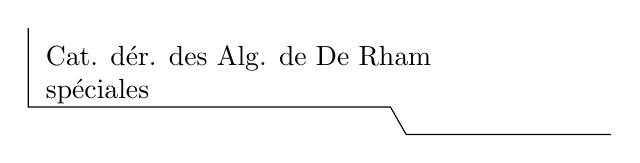
\begin{tikzpicture}
\node[anchor=west,align=left] at (.1,.4) {Cat. dér. des Alg. de De Rham\\spéciales};
\draw (0,1)--(0,0)--(4.6,0)--(4.8,-.35)--(7.4,-.35);
\end{tikzpicture}}}

Structure De Rham (à p.d. - sous-entendus)

Anneau bigradué [à degrés - total et ext - $\geq0$]\\
alterné pour degré ext
\[
A^{ij}\neq0\quad\deleted{\unsure{\Leftarrow}}\Rightarrow\unsure{q|0}\leq j\leq i
\]
degré complémentaire $=\unsure{j|i}-j\geq0$

différentiel [différentielle de bidegré $0,1$ ; c'est un diff. pour le degré ext $\unsure{j}$
\[
d(xy)=(dx)y+(-1)^{\deg.\mathrm{ext}\,x}x\,dy
\]
]

à p. div. sur l'idéal
\[
\sum_{i+j>0}A^{ij}=A^+
\]
[p.d. \deleted{\unsure{divisées}} compatibles aux $2$ grad
$\bigl(\gamma^d:A^{ij}\mathbin{-}A^{di,dj}\bigr)$
\deleted{\unsure{d}}
et la différentielle $(d\,x^{(i)}=x^{(i-1)}\,dx)$]

élément \uline{marqué}
$T\in Z^{10}(A^{**})\simeq H^{10}(A^{**})$

[Cohomologie $H^{*i}(A^{**})\simeq\unsure{h^i|h_i^i}\otimes_k k\{T\}$, \deleted{\unsure{où}}] $k=A^{00}$

Structure de De Rham \uline{spéciale} :
\[
\left\{\begin{array}{l}
k\{T\}\overset{\sim}{\longrightarrow}H^{*0}(A^{**})\\
H^{*i}(A^{**})=0\\
\text{les }A^{ij}\text{ sont }k\text{-plats}
\end{array}\right.
\]
[\uline{NB} c'est utile pour la stabilité par $\otimes_k k'$]

Structure de De Rham \uline{flasque} : les $A^{ij}$ pour $j<i$

\margin{$\unsure{)}\longrightarrow$ flasques.}
\margin{Univ. flasque : \deleted{stabilité par $\otimes_k\unsure{k'}$}}
\margin{\figure{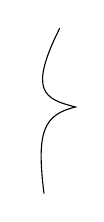
\begin{tikzpicture}
\draw (.2,1)..controls(-.2,.2)and(0,.1)..(.4,0)
..controls(0,-.1)and(-.1,-.3)..(0,-1.1);
\end{tikzpicture}}}

On parle de $k$-Structure de De Rham si $k=A^{00}$ \unsure{$\longrightarrow$|est} donné.

\deleted{$\unsure{\mathcal X}$}
$\mathcal X$, topos

\deleted{$\unsure{\mathcal{DR}}$}
$\mathcal{DR}_{sp}(\mathcal X,k)_0$ structures de De Rham spéciales sur $\mathcal X$ - avec comme flèches celles qui respectent \unsure{toutes|ttes} les structures \inserted{(y compris la structure $\unsure{u|k}$)}

$\mathcal{DR}_{spfl}(\mathcal X,\unsure{k})_0$ \quad `` \quad spéciales et flasques

$\mathcal{DR}_{spufl}(\mathcal X,\unsure{k})_0$ \quad `` \quad --- univ. flasques

$\mathcal{DR}_{sp}(\mathcal X,k)$, $\mathcal{DR}_{spfl}(\mathcal X,k)$, $\mathcal{DR}_{spufl}(\mathcal X,k)$

Catégories \inserted{de fractions} déduites en rendant inversibles ttes les flèches

- NB ce sont des quasi-isos -

\margin{93}
